
\documentclass[english,11pt]{exam}

% Appropriate definitions

\input exam_sty

\usepackage{amsmath,amssymb,babel,color,graphicx,latexsym,makeidx,marginnote}
\reversemarginpar

%% The spacing for maximal room on sheet
%\textheight 10in
%\textwidth  155mm

% change the following five definitions as needed
\newcommand{\Date}{15 May 2015}
\newcommand{\Time}{{\upshape 14h--17h}}
\newcommand{\Course}{Mathematical Models}
\newcommand{\CourseNumber}{201-225-AB}
\newcommand{\Instructor}{R.Masters}
\newcommand{\dsp}{\displaystyle}
\newcommand{\ds}{\displaystyle}
\newcommand{\vs}[1]{\vspace{#1in}}
\newcommand{\hs}[1]{\hspace{#1in}}
\usepackage{multicol}
\usepackage{tikz}
\usetikzlibrary{backgrounds} % Provides the framed and tight background options
                             % that show the bounding box.
\usetikzlibrary{intersections} % to compute intersections of paths
\usetikzlibrary{arrows}

% exam document class formatting commands
\extrawidth{1in}
\extraheadheight{-0.25in}
\extrafootheight{-0.375in}
\renewcommand{\questionlabel}{\bfseries\thequestion.} % bold question numbers
\pagestyle{headandfoot}
\lhead{Final Examination}
\chead{\CourseNumber}
\rhead{\Date}
\headrule 
%\lfoot{\iflastpage{Total: \numpoints~points}{}}
\cfoot{Page \thepage\ of \numpages}
%\rfoot{\iflastpage{This is the end of the examination.}{%
%  \ifincomplete{%
%    Question~{\IncompleteQuestion} continues on the next page.}{%
%    Please go on to the next page.}}}

% install fonts for the title page
\usepackage{oldgerm}
\newfont{\yinit}{yinit at 10pt}
\def\yinitial#1{
\hskip-2mm
\lower2mm
\hbox{\yinit #1}
\hskip-2mm}


% Start document

\begin{document}

\marksnotpoints
\pointsinmargin
\renewcommand{\marks}[1]
{\mbox{}\marginpar{\centering{(\,#1\,)}}\ignorespaces}
\begin{coverpages}

\begin{center}
\vspace*{-8ex}
\includegraphics[scale=0.25]{jaclogovertical.jpg}
\vskip 5ex \par
\scshape
{\huge%
\yinitial{D}epartment of%
\hskip .6em\yinitial{M}athematics \\[.67ex]
Final Examination}
\vskip 2ex \par
{\Large\upshape\Date\\[.67ex]\Time}
\vskip 1ex \par
{\huge \Course \vskip 1ex
\CourseNumber}
\vskip 5ex
\begin{minipage}[t]{6in}
\normalsize Instructor:\enspace
\hangindent = 1.15in
{\upshape \raggedright\Instructor}
\end{minipage}
\vskip 6ex
\begin{minipage}[t]{5in}
\normalsize \hbox to \textwidth
{Student name:\enspace\hrulefill}
\vskip 2ex
\hbox to \textwidth
{Student number:\enspace\hrulefill}
\vskip 2ex
\hbox to \textwidth
{Instructor:\enspace\hrulefill}
\vskip 2ex
\end{minipage}
\vskip 6ex
Instructions
\vskip 2ex
\begin{minipage}[t]{6.25in}
\begin{enumerate}\upshape
\item
Do not open this booklet before
the examination begins.
\item
Check that this booklet contains
{\numpages} \if\numpages1{page}\else{pages}\fi,
excluding this cover page and the formula sheet.
\item
Write all of your solutions in this booklet
and show all supporting work. 
%\item
%Give all answers in simplified exact form.
\item
If the space provided is not sufficient,
continue the solution on the opposite page. 
\end{enumerate}
\end{minipage}
\end{center}

\vskip 5ex

%\begin{center}
%\large\sffamily
%The use of calculators is neither needed nor permitted.
%\end{center}

\vfill

\end{coverpages}


\begin{questions}

%Question 1
\question  Find $\displaystyle y' $ for the following. \textbf{Do not simplify your answer.} 
\begin{parts}
\part [3] $\displaystyle y= \sin(\arctan (3x))+7^{2x}$
\vs{.1}
\part [3] $\displaystyle \arcsin (x+y)+2y =x^3$ \hspace{.25cm} Hint: Solve for $y'$.
\vs{.1}
\part [3] $\displaystyle y=\int_{\cos x}^1 (-2t+3\sin t)\;dt$ \hspace{.25cm} Hint: use part 1 of the  F.T.C. 
\vs{.1}
\part [3] $\displaystyle y= \log_7(\tan x)+e^{\sec5x}$
\vs{.1}
\end{parts}

%Question 2
\question
Given $\dsp f(x)= \frac{x}{x^2-9}$ \hs{.25} $\dsp f'(x)=-\frac{(x^2+9)}{(x^2-9)^2}$ \hs{.25}  $\dsp f''(x)=\frac{(2x)(x^2+27)}{(x^2-9)^3}$.\\
 Find (if any):
\begin{multicols}{2}
\begin{parts}
\part [1] The $x$ and $y$ intercept(s).
\part [1] The vertical and horizontal\\ asymptotes.
\part [1] The critical numbers
\part [1] The inflection points.
\part [1] Local (relative) extrema.
\part [1] Intervals of upward or downward\\ concavity.
\part [1] Intervals on which $f$ is increasing or\\ decreasing.
\part [3] Sketch the graph of $f$.
\end{parts}
\end{multicols}
\vs{.1}


%Question 3 
\question[4]
Use Simpson's Rule with $n=4$ to estimate the value of $\displaystyle\int_{1}^5\frac{1}{x^2+x}\;dx$ (give your answer to 3 decimals).  
\vs{.1}

%Question 4
\question [5]

The illumination of an object (O) by a light source is directly proportional to the strength of the source and inversely proportional to the square of the distance from the source. If two light sources ($S_1$ and $S_2$), one 8 times as strong as the other, are placed 100 ft apart, how many feet from the brighter source should an object be placed on the line between the sources so as to receive the least illumination (see diagram below)?


\definecolor{xdxdff}{rgb}{0.49019607843137253,0.49019607843137253,1.0}
\definecolor{qqqqff}{rgb}{0.0,0.0,1.0}
\begin{tikzpicture}[line cap=round,line join=round,>=triangle 45,x=1.0cm,y=1.0cm]
\clip(2.64,0.719999999999999) rectangle (7.54,2.579999999999999);
\draw (3.0,1.74)-- (7.0,1.74);
\draw (3.0,1.8)-- (3.0,1.32);
\draw (7.0,1.8)-- (7.0,1.32);
\draw (3,1.32)-- (7.0,1.32);
\draw (4.4,1.3) node[anchor=north west] {$100 ft$};
\begin{scriptsize}
\draw [fill=qqqqff] (3.0,1.74) circle (1.5pt);
\draw[color=qqqqff] (3.0,2.0) node {$S_1$};
\draw [fill=qqqqff] (7.0,1.74) circle (1.5pt);
\draw[color=qqqqff] (7.0,2.0) node {$S_2$};
\draw[color=black] (4.2,2.0) node {$O$};
\draw [fill=xdxdff] (4.18,1.7399999999999998) circle (1.5pt);
\end{scriptsize}
\end{tikzpicture}
\vs{.1}

%Question 5
\question [4]
\begin{multicols}{2}
 Find the area of the region between the two graphs, $\dsp f(x)=(x-1)^3$ and $\dsp g(x)= x-1$. 
\definecolor{uuuuuu}{rgb}{0.26666666666666666,0.26666666666666666,0.26666666666666666}
\begin{tikzpicture}[line cap=round,line join=round,>=triangle 45,x=1.0cm,y=1.0cm]
\draw[->,color=black] (-0.86,0.0) -- (2.74,0.0);
\foreach \x in {1,2}
\draw[shift={(\x,0)},color=black] (0pt,2pt) -- (0pt,-2pt) node[below] {\footnotesize $\x$};
\draw[->,color=black] (0.0,-1.6600000000000001) -- (0.0,1.6400000000000001);
\foreach \y in {-1,1}
\draw[shift={(0,\y)},color=black] (2pt,0pt) -- (-2pt,0pt) node[left] {\footnotesize $\y$};
\draw[color=black] (0pt,-10pt) node[right] {\footnotesize $0$};
\clip(-0.86,-1.6600000000000001) rectangle (2.74,1.6400000000000001);
\draw[smooth,samples=100,domain=-0.86:2.74] plot(\x,{((\x)-1.0)^(3.0)});
\draw[smooth,samples=100,domain=-0.86:2.74] plot(\x,{(\x)-1.0});
\draw (1.7,0.8200000000000001) node[anchor=north west] {$f(x)$};
\draw (0.3,-0.4) node[anchor=north west] {$g(x)$};
\draw (-0.44,1.7) node[anchor=north west] {$y$};
\draw (2.3000000000000003,-0.1) node[anchor=north west] {$x$};
\begin{scriptsize}
\draw[color=black] (-0.12,-2.34) node {$f$};
\draw[color=black] (-1.34,-2.34) node {$g$};
\draw [fill=uuuuuu] (0.0,-1.0) circle (1.5pt);
\draw [fill=uuuuuu] (1,0) circle (1.5pt);
\draw [fill=uuuuuu] (2.0,1.0) circle (1.5pt);
\end{scriptsize}
\end{tikzpicture}
\end{multicols}
\vs{.1}


%Question 6
\question Evaluate the following limits. 
\begin{parts}
\part[3] $\dsp \lim_{x \rightarrow \frac{\pi}{2}} (1-\sin x)\cdot \tan x$
\vs{.1}
\part[3] $\dsp \lim_{x\rightarrow 0} \frac{e^x+e^{-x}-2}{1-\cos 2x}$
\vs{.1}
\part[4] $\dsp \lim_{x \rightarrow 0} \left(\frac{1}{x}\right)^{\sin x}$ 
\vs{.1}
\end{parts}

%Question 7
\question [3] 
Boyle's Law states that when a sample of gas is compressed at a constant temperature, the pressure \(P\) and the volume \(V\) satisfy the equation \(PV=C\), where \(C\) is a constant. Suppose that at a certain instant the volume is \(600\,cm^3\), the pressure is \(150\,kPa\), and the pressure is increasing at a rate of \(20\,kPa/min\). At what rate is the volume decreasing at this instant?
\vs{.1} 

%Question 8
\question Solve the following differential equations for y.
\begin{parts}
\part[3]
$\dsp y dt + t dy = 3ty\; dt $  \hs{.75} with initial condition y(1)=1.
\vs{.1}
\part[3]
$\dsp (yx^2+y)\frac{dy}{dx}=\tan^{-1}x$  
\end{parts}
\vs{.1}

%Question 9
\question [4]  Find the volume of the solid formed by rotating the region enclosed by \[x=0, \ x=1, \ y=0, \ y= 6 +x^{6}\]
about the \(y\)-axis. \hspace{.25cm} Hint: Split the region into two. 

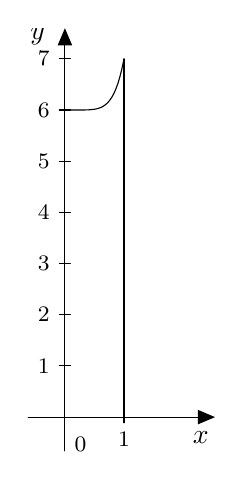
\begin{tikzpicture}[line cap=round,line join=round,>=triangle 45,x=.75cm,y=.65cm]
\draw[->,color=black] (-0.6212870623728584,0.0) -- (2.5415165307860317,0.0);
\foreach \x in {,1,}
\draw[shift={(\x,0)},color=black] (0pt,2pt) -- (0pt,-2pt) node[below] {\footnotesize $\x$};
\draw[->,color=black] (0.0,-0.6604601280001708) -- (0.0,7.598402281444725);
\foreach \y in {,1,2,3,4,5,6,7}
\draw[shift={(0,\y)},color=black] (2pt,0pt) -- (-2pt,0pt) node[left] {\footnotesize $\y$};
\draw[color=black] (0pt,-10pt) node[right] {\footnotesize $0$};
\clip(-0.6212870623728584,-0.6604601280001708) rectangle (2.5415165307860317,7.598402281444725);
\draw[smooth,samples=100,domain=0.0:1.0] plot(\x,{6.0+(\x)^(6.0)});
\draw (1.0,7.0)-- (1.0,0.0);
\draw (-0.75,7.8) node[anchor=north west] {$y$};
\draw (2.0,-0.1) node[anchor=north west] {$x$};
\end{tikzpicture}
\vs{.1}

%Question 10
\question[3]
Determine if $\dsp y=x^3 +2x^2-5$ is a solution to the differential equation $\dsp -y'''+y''-\frac{y'}{x}=3x-6$
\vs{.1}

%Question 11
\question
Integrate the following integrals. 

\begin{parts}
\part[4]
$\ds\int \frac{\cos(\ln x)}{x} \;dx$
\vs{.1}
\part[4]
$\displaystyle\int \tan^3 x\;dx$
\vs{.1}
\part[4]
$\displaystyle\int \frac{1}{\sqrt{x^2+6x+13}}\;dx$
\vs{.1}
\part[4]
$\displaystyle\int \frac{5}{x^2-9}\;dx$
\vs{.1}
\part[4]
$\displaystyle\int \tan^9 x\sec^4 x\;dx$
\vs{.1}
\part[4]
$\dsp \int \arcsin x\; dx$
\vs{.1}
\part[4]
$\dsp \int \sin^2(2x)\; dx$
\vs{.1}
\end{parts}

%Question 12
\question [5]  Solve the following first order linear differential equation for y.\\ 
$\dsp \frac{dy}{dx}+2y\cot x=4\cos x$  \hs{.75} with initial condition $\dsp x=\pi/2$ when $\dsp y=1/3$ 
\vs{.1}

%Question 13
\question Given the function and its graph. 
\begin{multicols}{2}
\[
f(x) = \begin{cases} 2, & \text{if $-\pi\le x<-\frac{\pi}{2}$\;\;, $\frac{\pi}{2}\le x<\pi$}\\
3,\;\;\; & \text{if $-\frac{\pi}{2}\le x < \frac{\pi}{2}$}\\
\end{cases}
\]\\
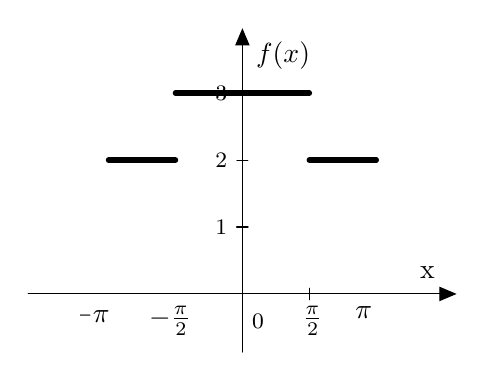
\begin{tikzpicture}[line cap=round,line join=round,>=triangle 45,x=.85cm,y=.85cm]
\draw[->,color=black] (-3.2,0) -- (3.2,0);
\foreach \x in {,,,}
\draw[shift={(\x,0)},color=black] (0pt,2pt) -- (0pt,-2pt) node[below] {\footnotesize $\x$};
\draw[color=black] (2.51,0.08) node [anchor=south west] { x};
\draw[->,color=black] (0,-0.87) -- (0,3.97);
\foreach \y in {,1,2,3}
\draw[shift={(0,\y)},color=black] (2pt,0pt) -- (-2pt,0pt) node[left] {\footnotesize $\y$};
\draw[color=black] (0.06,3.56) node [anchor=west] { $f(x)$};
\draw[color=black] (0pt,-10pt) node[right] {\footnotesize $0$};
\clip(-2.42,-0.87) rectangle (2.7,3.97);
\draw [line width=2pt] (-1,3)-- (1,3);
\draw [line width=2pt] (-2,2)-- (-1,2);
\draw [line width=2pt] (1,2)-- (2,2);
\draw (-2.7,-0.04) node[anchor=north west] {$-\pi$};
\draw (-1.54,-0.04) node[anchor=north west] {$-\frac{\pi}{2}$};
\draw (0.75,-0.04) node[anchor=north west] {$\frac{\pi}{2}$};
\draw (1.54,-0.04) node[anchor=north west] {$\pi$};
\end{tikzpicture}
\end{multicols}
\begin{parts}
\part[2] Determine if the function is even or odd. \hs{.1}Show your work or Explain to obtain full marks
\vs{.1}
\part[4]
Find the first three non-zero terms of the  Fourier series for the function above.  
Hint: find $\dsp a_0,a_1,a_2,a_3,\dotsc,b_1,b_2,\dotsc$ and write the function expansion.
\end{parts}

\end{questions}

\textbf{Answers}

\begin{questions}

\question 
\begin{parts}
\part
$\displaystyle y'=\cos(\arctan 3x)\cdot \frac{3}{1+(3x)^2}+2\cdot7^{2x}\cdot \ln 7$
\part
$\displaystyle y'=\frac{3x^2\sqrt{1-(x+y)^2}-1}{1+2\sqrt{1-(x+y)^2}}$
\part
$\displaystyle y'=\frac{\sec^2x}{\tan x\cdot \ln 7}+e^{\sec 5x}\cdot 5\sec 5x \tan 5x$
\part
$\displaystyle y'=(2\cos x -3\sin(\cos x))( -\sin x)$
\end{parts}

\question
$\dsp A \approx 0.522$

\question 
\begin{parts}
\part
$\displaystyle x$-int $=0$ and $\dsp y$-int $=0$
\part
V.A. $x = \pm 3$ ; H.A. $y = 0$
\part
None
\part
$x=0$
\part
None
\part
C.U. $\ds ]-3,0[ \cup ]3,\infty[$  
\\
C.D. $\dsp ]-\infty,-3[ \cup ]0,3[$
\part
Inc. No where\\
dec. $\ds ]-\infty, \infty[$
\end{parts}

\question
$\ds \frac{200}{3}ft$ away from source 2

\question
$\ds A =$ 1/2

\question 
\begin{parts}
\part
$\ds 0$
\part
1/2
\part
$\ds 1$
\end{parts}

\question 
$\ds \frac{dV}{dt}=-80$ cm$^3$/min

\question
\begin{parts}
\part
$\ds y=\frac{e^{3(t-1)}}{t}$
\part
$\ds y=\sqrt{(\arctan x)^2+2c}$
\end{parts}

\question
$\ds \frac{25}{4}\pi$

\question
yes

\question
\begin{parts}
\part
$\ds \sin(\ln x)+c$
\part
$\ds \frac{\tan^2 x}{2}-\ln |\sec x|+c$
\part
$\ds \ln\left|\frac{\sqrt{x^2+6x+13}+x+3}{2}\right|+c$
\part
$\ds \ln \left| \frac{x-3}{x+3}\right|^{5/6}+c$
\part
$\ds \frac{\tan^{12}x}{12}+\frac{\tan^{10}x}{10}+c$
\part
$\ds x\cdot \arcsin x +\sqrt{1-x^2}+c$
\part
$\ds 1/2 \left(x-1/4\sin x \right) +c$
\end{parts}

\question
$\ds y=4/3\sin x-\csc^2x$

\question
\begin{parts}
\part
$\ds f(x)$ is even
\part
$\ds f(x)= \frac{5}{2}+\frac{2}{\pi}\cos x-\frac{2}{3\pi}\cos x+\frac{2}{5\pi}\cos x-\dotsb$
\end{parts}
\end{questions}


\end{document}

\end
